\documentclass[12pt, a4paper, oneside]{ctexart}
\usepackage{amsmath, amsthm, amssymb, bm, color, framed, graphicx, hyperref, mathrsfs}

\title{\textbf{10月29日作业}}
\author{韩岳成 524531910029}
\date{\today}
\linespread{1.5}
\definecolor{shadecolor}{RGB}{241, 241, 255}
\newcounter{problemname}
\newenvironment{problem}{\begin{shaded}\stepcounter{problemname}\par\noindent\textbf{题目\arabic{problemname}. }}{\end{shaded}\par}
\newenvironment{solution}{\par\noindent\textbf{解答. }}{\par}
\newenvironment{note}{\par\noindent\textbf{题目\arabic{problemname}的注记. }}{\par}

\begin{document}

\maketitle

\begin{problem}
    设随机变量$(X,Y)$的联合概率密度为

    $$f(x,y)=\begin{cases}\dfrac{3}{4}x\:,&\quad0\leqslant x\leqslant2\:,0\leqslant y\leqslant\dfrac{x}{2}\:,\\0\:,&\quad\text{其他}.\end{cases}$$

    (1)求$(X,Y)$的边缘概率密度; 

    (2)试问$X$与$Y$是否相互独立?
\end{problem}

\begin{solution}
    (1) 由联合概率密度可得
    \[f_X(x)=\int_{0}^{\frac{x}{2}} \frac{3}{4}x \, dy = \frac{3}{8}x^2, \quad 0 \leq x \leq 2,\]
    \[f_Y(y)=\int_{2y}^{2} \frac{3}{4}x \, dx = \dfrac{3}{2} - \dfrac{3}{2}y^2, \quad 0 \leq y \leq 1.\]
    因此边缘概率密度为
    \[f_X(x)=\begin{cases}\dfrac{3}{8}x^2\:,&\quad0\leqslant x\leqslant2\:,\\0\:,&\quad\text{其他},\end{cases}\]
    \[f_Y(y)=\begin{cases}\dfrac{3}{2} - \dfrac{3}{2}y^2\:,&\quad0\leqslant y\leqslant1\:,\\0\:,&\quad\text{其他}.\end{cases}\]
    (2) $f_X(x)f_Y(y) \neq f(x,y)$,因此$X$与$Y$不相互独立。
\end{solution}

\begin{problem}
设随机变量($X,Y)$的联合概率密度为
$$f(x,y)=\begin{cases}x+y,&\quad0<x<1,0<y<1,\\0,&\quad\text{其他}.\end{cases}$$
求在$\left\{0<X<\frac1n\right\}$的条件下$Y$的条件分布函数.
\end{problem}

\begin{solution}
由联合概率密度可得
\begin{align*}
    F_{Y|X}(y|0<X<\tfrac{1}{n}) &= P(Y \leq y | 0 < X < \tfrac{1}{n}) \\
    &= \frac{P(Y \leq y, 0 < X < \tfrac{1}{n})}{P(0 < X < \tfrac{1}{n})}\\
    &= \frac{\int_0^{\frac{1}{n}} \int_{-\infty}^y (x + t) \, dt \, dx}{\int_{0}^{\frac{1}{n}} \int_{-\infty}^{+\infty} (x + t) \, dt \, dx} \\
    &=\begin{cases}0,&y<0,\\\frac{\int_0^{\frac{1}{n}} \int_{0}^y (x + t) \, dt \, dx}{\int_{0}^{\frac{1}{n}} \int_{0}^{1} (x + t) \, dt \, dx},&0\leq y < 1,\\1,&y\geq1.\end{cases}\\
    &=\begin{cases}0,&y<0,\\\frac{y\left(1+ny\right)}{1+n},&0\leq y<1,\\1,&y\geq1.\end{cases}
\end{align*}

\end{solution}

\begin{problem}
设随机变量(X,Y)的联合分布律为
\begin{center}
    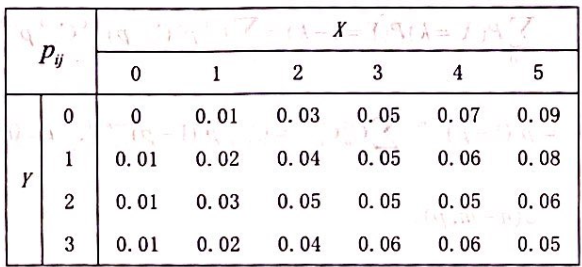
\includegraphics[width=0.45\textwidth]{image.png}
\end{center}
分别求$Z=X+Y$、$M=\max\{X,Y\}$和$N=\min\{X,Y\}$的分布律.
\end{problem}

\begin{solution}
由联合分布律可得

\begin{tabular}
{|c|c|c|c|c|c|c|c|c|c|}
    \hline
    $Z$ & 1 & 2 & 3 & 4 & 5 & 6 & 7 & 8 \\
    \hline
    $P(Z=z)$ & $0.02$ & $0.06$ & $0.13$ & $0.19$ & $0.24$ & $0.19$ & $0.12$ & $0.05$ \\
    \hline
\end{tabular}
\vspace{0.5cm}

\begin{tabular}
{|c|c|c|c|c|c|}
    \hline
    $M$ & 1 & 2 & 3 & 4 & 5\\
    \hline
    $P(M=m)$ & $0.04$ & $0.16$ & $0.28$ & $0.24$ & $0.28$ \\
    \hline
\end{tabular}
\vspace{0.5cm}

\begin{tabular}
    {|c|c|c|c|c|}
    \hline
    $N$ & 0 & 1 & 2 & 3 \\
    \hline
    $P(N=n)$ & $0.28$ & $0.30$ & $0.25$ & $0.17$ \\
    \hline
\end{tabular}
\end{solution}

\begin{problem}
    设随机变量$ X $与$ Y $相互独立,且服从相同的分布,其中 $P(X=1)=p$, $P(X=0)=1-p$, 令
    \[Z=\begin{cases} 1, & \text{若 X+Y 为偶数}, \\ 0, & \text{若 X+Y 为奇数}, \end{cases}\]
    问$p$取何值时$ X $与$ Z $相互独立?
\end{problem}
\begin{solution}
    由题意可得
    \[P(Z=1)= P(X=0, Y=0) + P(X=1, Y=1) = (1-p)^2 + p^2 = 1 - 2p + 2p^2,\]
    \[P(Z=0)= P(X=0, Y=1) + P(X=1, Y=0) = 2p(1-p) = 2p - 2p^2.\]
    因为$X$与$Z$相互独立,所以
    \[P(X=1, Z=1) = P(X=1, Y=1) = p^2 = P(X=1)P(Z=1) = p(1 - 2p + 2p^2).\]
    解得$p = \frac{1}{2}$,即当$p = \frac{1}{2}$时,$X$与$Z$相互独立。
\end{solution}

\begin{problem}
设二维随机变量(X,Y)的联合概率密度为
$$f(x,y)=\begin{cases}
1, & 0<x<1,0<y<2x, \\
0, & \text{其他.}
\end{cases}$$
令$Z=2X-Y$,求$Z$的概率密度$f_{Z}(z)$.
\end{problem}
\begin{solution}
由题意可得
\[
Z=2X-Y \Rightarrow Y=2X-Z.
\]
因此
\[
f_{Z}(z)=\int_{0}^{1} f(x, 2x-z) \, dx.
\]
当$0<x<1$且$0<y<2x$时,$0<2x-z<2x$,即$z<2x$,所以
\[
f_{Z}(z)=\int_{\frac{z}{2}}^{1} 1 \, dx = 1 - \frac{z}{2}, \quad 0<z<2.
\]
因此
\[
f_{Z}(z)=\begin{cases}
1 - \frac{z}{2}, & 0<z<2, \\
0, & \text{其他.}
\end{cases}
\]
\end{solution}

\begin{problem}
设$X$与$Y$是相互独立且同分布的随机变量,其概率密度为

$$f_X(x)=\begin{cases}\dfrac{10}{x^2},&\quad x>10\:,\\0\:,&\quad x\leqslant10\:,\end{cases}$$

求 $Z=\frac XY$的概率密度。
\end{problem}

\begin{solution}
由变量变换 $x=zy$,得到
\[
f_Z(z)=\int_{y>0} f_X(zy) f_Y(y) |y|\,\mathrm{d}y.
\]

由于 $X>10, Y>10$,

若 $0<z<1$,则 $zy>10 \Rightarrow y>10/z > 10$,积分下限 $y=10/z$:
\[
f_Z(z)=\int_{10/z}^{\infty} \frac{10}{(zy)^2} \cdot \frac{10}{y^2} \cdot y \, \mathrm{d}y
= \int_{10/z}^{\infty} \frac{100}{z^2 y^3} \, \mathrm{d}y
= \frac{50}{z^2 (10/z)^2} = \frac{1}{2}.
\]

若 $z\ge 1$,则 $zy>10 \Rightarrow y>10$,积分下限 $y=10$:
\[
f_Z(z)=\int_{10}^{\infty} \frac{100}{z^2 y^3} \, \mathrm{d}y
= \frac{50}{z^2 \cdot 10^2} = \frac{1}{2 z^2}.
\]


因此 $Z$ 的概率密度为
\[
f_Z(z)=
\begin{cases}
\dfrac{1}{2}, & 0<z<1,\\[2mm]
\dfrac{1}{2z^2}, & z\ge 1,\\[1mm]
0, & \text{其他}.
\end{cases}
\]
\end{solution}

\begin{problem}
设$(X,Y)$在区域$D=\{(x,y)\mid x\leq y\leq 2\}$内均匀分布,$Z=g(X,Y)=\begin{cases}0,Y<1\\Y,Y\geq1\end{cases}$,求$Z$的分布函数。
\end{problem}

\begin{solution}
由题意可得区域$D$的面积为
\[S_D=\int_{-\infty}^{+\infty}\int_{x}^{2} 1 \, dy \, dx = \int_{-\infty}^{2} (2 - x) \, dx = 2(2) - \frac{(2)^2}{2} = 2.\]
因此$(X,Y)$的分布函数为
\[f_{X,Y}(x,y) = \begin{cases} \frac{1}{2}, &x\leq y \leq 2\\ 0, & \text{其他.} \end{cases}\]
当$z<0$时,$F_Z(z)=0$;

当$0 \leq z < 1$时,
\[P(z=0) = \frac12P(y<1) = \frac12\int_0^1\int_0^y dxdy = \frac14,\]
因此$F_Z(z) = \frac14$;

当$1 \leq z < 2$时,
\[P(Z\leq z) = \frac12P(y<z) = \frac12\int_0^z\int_0^y dxdy = \frac{z^2}{4},\]
因此$F_Z(z) = \frac{z^2}{4}$;

当$z \geq 2$时,$F_Z(z) = 1$。
综上所述,$Z$的分布函数为
\[F_Z(z) = \begin{cases} 0, & z<0,\\ \frac14, & 0 \leq z < 1,\\ \frac{z^2}{4}, & 1 \leq z < 2,\\ 1, & z \geq 2. \end{cases}\]
\end{solution}
\end{document}